\section{Plan de trabajo}

\subsection{Perfil de Poiseuille}

Se busca que en la confluencia exista un flujo de entrada con régimen laminar. Para ello se escoge como volumen de control la entrada de la tubería, como se muestra en la Figura \ref{f2}. La condiciones de contorno son: 
\begin{itemize}
\item Velocidad entrada constante en la entrada
\item Condición de flujo nulo en la salida ($\partial u / \partial x = 0 \rightarrow u = cte$)
\end{itemize}

Utilizando la metodología antes expuesta se busca calcular el perfil de velocidad a la salida del volumen de control. Una vez obtenido el perfil de velocidad se puede trabajar en la confluencia

\begin{figure}[H]
\centering
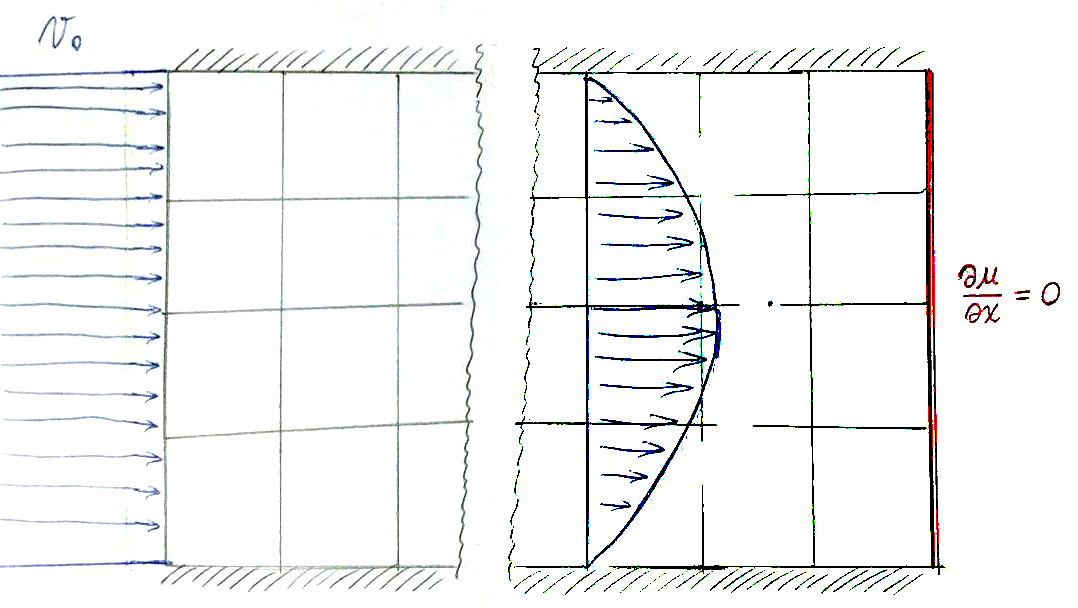
\includegraphics[width=0.8\textwidth]{f2.png}
\caption{ } \label{f2}
\end{figure}

\subsection{Confluencia}

Con el perfil de velocidad previamente calculado a la salida de la tubería, naturalmente se impone el mismo perfil como condición de entrada en la confluencia en ambos extremos, como se ve en la Figura \ref{f3}. De esta manera la resolución del problema es computacionalmente más sencilla y sin perder sustento físico. \\

Se resuelve el campo de velocidad dentro del volumen de control $\Omega$. Conociendo el $\vec{v}$ en cada punto se emplea la ecuación de conservación/transporte de un escalar pasivo (ecuación (\ref{transporte})). Por ejemplo, se puede imponer $C=0$ en $t=0$, y tener un sumidero constante $C=1$ en una o en las dos entradas de la confluencia (ver Figura). Calcular el campo $C(x,y)$ permite visualizar el comportamiento del fluido.

\begin{figure}[H]
\centering
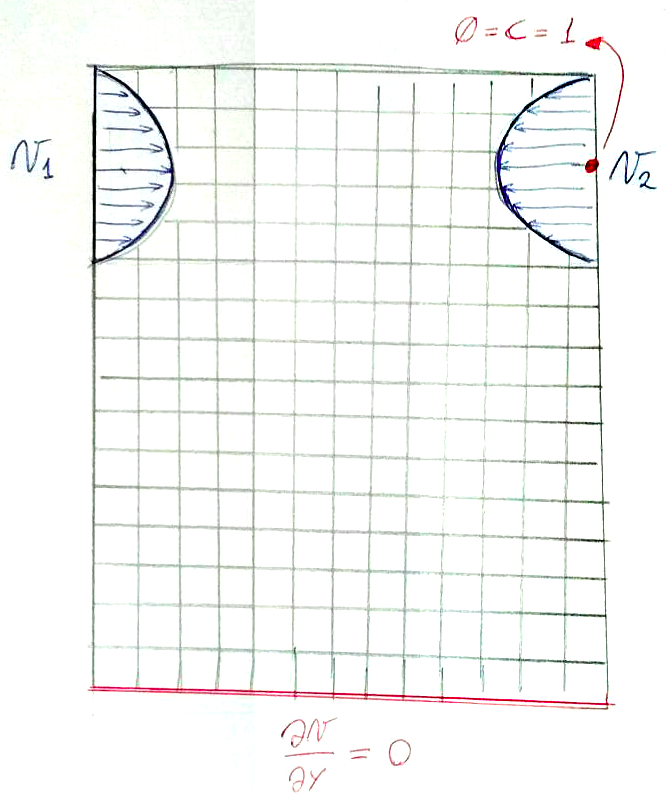
\includegraphics[width=0.8\textwidth]{f3.png}
\caption{ } \label{f3}
\end{figure}